\section{Test}
The corpus we use comprise of three different speakers: two men and one woman.
Each speaker has 460 samples, where the average duration of each sample is
about 4 seconds.  For each speaker, we randomly choose $M$ samples to train GMM
model. For more deep inspection of the algorithm, M is enumerated from 2 to 5.
We then feed the whole corpus to to the algorithm, and test its accuracy.
Further more, for the robustness of the result, we repeat the test process 10
times, and average the result.

\subsection{Result}
\begin{figure}[!ht]
\centering
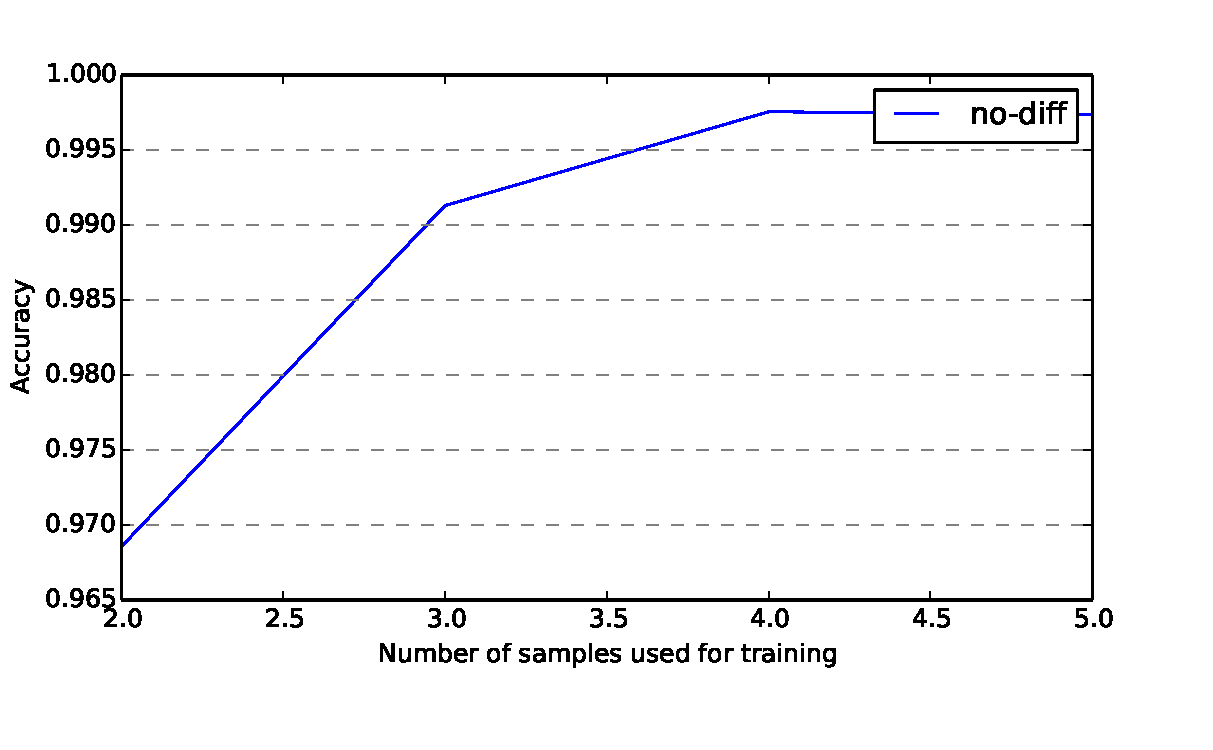
\includegraphics[width=\textwidth]{res/plot.pdf}
\caption{Accuracy vs Number of samples used for training}
\label{fig:result}
\end{figure}

\begin{table}[!ht]
	\centering
	\begin{tabular}{|c|c|c|c|c|}
		\hline
        \#Training sample & 2 & 3 & 4 & 5 \\\hline
		Accuracy & 0.968555 & 0.991293 & 0.997549 & 0.997380 \\\hline
	\end{tabular}
	\label{table:result}
\end{table}

As we can see from the curve ploted, the performance of the algorithm increases as
the number of training samples given increases. The accuracy when
just using two training samples for each user has reached $96.55\%$, which
is supprisingly high with respect to using such small amount of training samples.

When using 4 to 5 samples per speaker, the accuracy is above $99.73\%$, which
strongly confirmed the effectivenes of MFCC feature and GMM modeling for each
speaker.

However, further inspection on misclassified samples showed limitation on our
test case: all the misclassified samples are within two men speakers, indicates
the weakness of the algorithm.
